\documentclass{article}
\textwidth=6in
\hoffset=0in
\voffset=0in

\usepackage[a4paper, total={6in, 8in}]{geometry}
\usepackage{amsmath}
\usepackage{amssymb}
\usepackage{stmaryrd}
\usepackage{graphicx}
\usepackage{tikz}
\usetikzlibrary{automata, arrows}
\usepackage{pifont}
\usepackage{amssymb}
\usepackage{gensymb}
\usepackage{ngerman}
\usepackage[ampersand]{easylist}

% needs to be updated
\author{Max Springenberg, 177792}
\title{\
    }
\setcounter{section}{2}
\date{}

% custom commands
% \Theta \Omega \omega
\newcommand{\tab}{\null\ \qquad}
\newcommand{\gap}{\null\ \\ \\}
\newcommand{\lA}{\leftarrow}
\newcommand{\rA}{\rightarrow}
\newcommand{\ue}{\infty}
\newcommand{\eps}{\epsilon}
\newcommand{\task}[1]{\textbf{#1} \\ \gap}
\newcommand{\cmark}{\ding{51}}
\newcommand{\xmark}{\ding{55}}
\newcommand{\degr}{\degree}

% content
\begin{document}
% title page
\maketitle
\newpage
% actual paper

\task{3.2 c)}
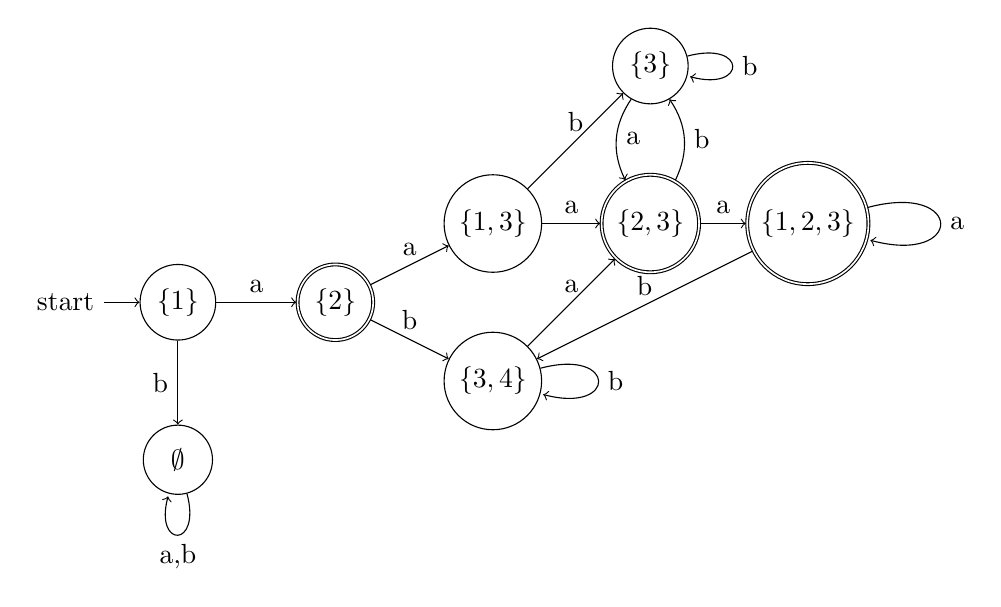
\begin{tikzpicture}
    \node[initial, state]   (1)     at (0,0){$\{1\}$};
    \node[accepting, state] (2)     at (2,0){$\{2\}$};
    \node[state]            (13)    at (4,1){$\{1,3\}$};
    \node[state]            (34)    at (4,-1){$\{3,4\}$};
    \node[state]            (3)     at (6,3){$\{3\}$};
    \node[accepting, state] (23)    at (6,1){$\{2,3\}$};
    \node[accepting, state] (123)   at (8,1){$\{1,2,3\}$};
    \node[state]            (empty) at (0,-2){$\emptyset$};
    \path
        (1)
            edge [->, above] node {a} (2)
            edge [->, left] node {b} (empty)
        (2)
            edge [->, above] node {a} (13)
            edge [->, above] node {b} (34)
        (13)
            edge [->, above] node {a} (23)
            edge [->, above] node {b} (3)
        (23)
            edge [->, above] node {a} (123)
            edge [->, bend right, right] node {b} (3)
        (123)
            edge [->, loop right] node {a} (123)
            edge [->, above] node {b} (34)

        (empty)
            edge [->, loop below] node {a,b} (empty)
        (34)
            edge [->, above] node {a} (23)
            edge [->, loop right] node {b} (34)
        (3)
            edge [->, bend right, right] node {a} (23)
            edge [->, loop right] node {b} (3)
       ;
\end{tikzpicture}\\
\end{document}
